\subsection{Depth Sensors}

Depth sensors play an increasingly important role in modern robotic applications.
They give a robot a fast mean to detect obstacles and locate itself in its environment.
The following paragraphs describe the underlying sensor principles for the depth sensors used in this thesis, but does not introduce the general area of depth sensing\cite{blais_2003}.

\subsubsection{Structured-Light Depth Sensors}

\begin{figure}[H]
    \centering
    \begin{subfigure}[t]{0.45\textwidth}
        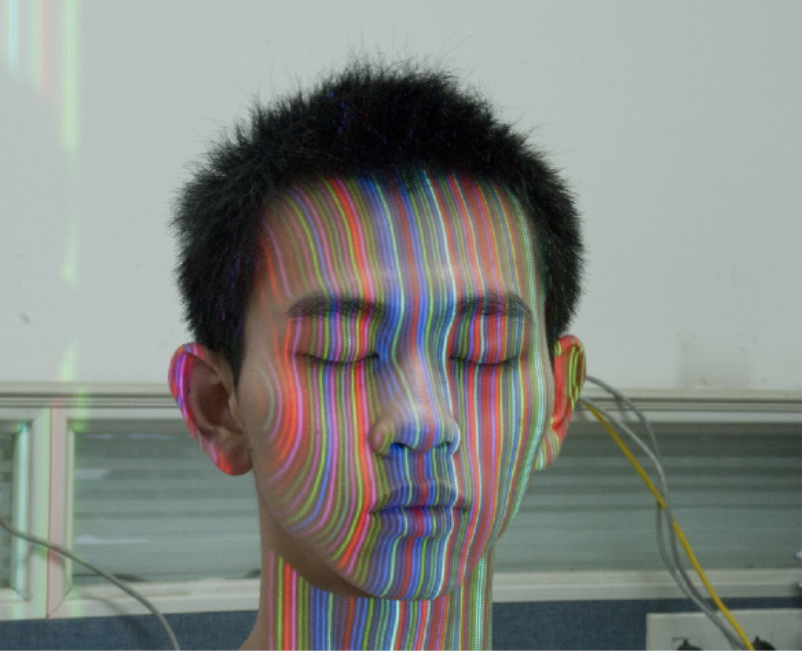
\includegraphics[width=\textwidth]{chapter03/img/depth_pattern_face.png}
        \caption{Structured light depth sensors project a predefined light pattern into the environment and observe the deformation of that pattern\cite{sl_depthsensor_calibration}.}
    \end{subfigure}
    \begin{subfigure}[t]{0.45\textwidth}
        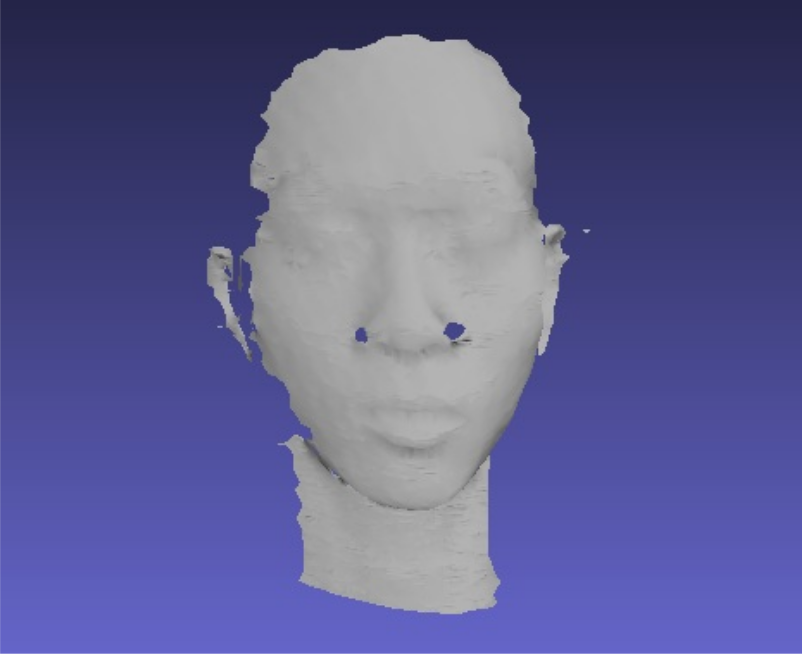
\includegraphics[width=\textwidth]{chapter03/img/depth_face_reconstructed.png}
        \caption{This figure shows the reconstruction result of the scanned face scanned\cite{sl_depthsensor_calibration}.}
    \end{subfigure}
    \caption[Demonstration of visible light patterns used for structured-light depth sensors]{One way to reconstruct depth information are structured light depth sensors. A predefined light pattern is projected into space. As the photons reflect from obstacles at different distances relative to the observer, the light pattern appears transformed. This deformation is used to reconstruct the geometry of the objects. The light emitted is usually not visible to humans as infrared light sources and cameras are commonly used in robotic applications.\label{fig:sl_face}}
\end{figure}
Structured-light depth sensor project a known light pattern into space and optically sense the reflections.
From a viewpoint different then the projector the pattern appears distorted, due to the shape of the reflecting object.
Stripes and grids of lines or points are commonly used for sensors in robotic applications, such as the Kinectv1 and Intel RealSense sensors.
Sensing the projected patterns from multiple viewpoints allows triangulation techniques to recover the depth information.
Using specialized processing hardware, built into the sensing system, mobile robotic depth sensors achieve framerates of 30fps or more.

\subsubsection{\acrlong{ToF}-Cameras}

\begin{figure}[H]
    \centering
    \begin{subfigure}[t]{0.45\textwidth}
        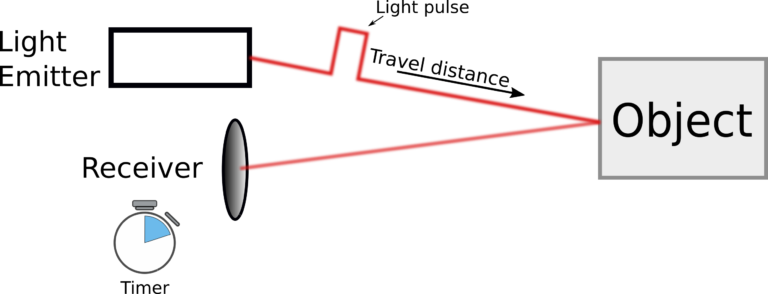
\includegraphics[width=\textwidth]{chapter03/img/tof_traveltime_original.png}
        \caption{One way to measure the time-of-flight for photons is to emit a light pulse and measure the roundtrip time until sensing. Illustration adopted from\cite{tof_cameras}.}
    \end{subfigure}
    \begin{subfigure}[t]{0.45\textwidth}
        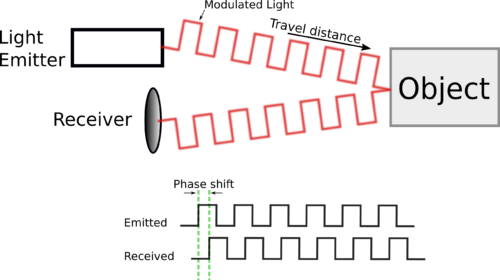
\includegraphics[width=\textwidth]{chapter03/img/tof_phase_shift_original.png}
        \caption{The second, more recent approach is measuring the phase-shift of photons relative to the light source. This allows a continously emitting light source. Illustration adopted from\cite{tof_cameras}.}
    \end{subfigure}
    \caption[Illustration of two commonly used measuring principle for Time-of-Flight cameras]{Measuring the distance of objects via time-of-flight\label{fig:tof_illustration}}
\end{figure}

\begin{itemize}
    \item range imaging camera system to measure the distance of world point by measuring the time, light needs to travel to the object and back for every pixel of an image
    \item the light source can be a laser or a LED
    \item the technology is related to \acrshort{LIDAR}
    \item these camera systems operate faster than \acrshort{LIDAR} but have lower resolution
    \item especially in robotics the kinect v2 is commonly found as time-of-flight sensor
    \item phase-shift reduces range of measurement to a few meters, depending on the wavelength of the used light
\end{itemize}

\subsubsection{\acrlong{LIDAR}}

\acrlong{LIDAR} (\acrshort{LIDAR}) uses the same measurement principle as \acrshort{ToF}-Cameras, it measures the distance of an object using time measurements.
The difference between \acrshort{LIDAR} and \acrshort{ToF}-Cameras is the usage of a \acrshort{laser} as light source.
The most common configurations use a horizontally rotating mirror that reflects the beam into the room.
For vertical coverage measurement head is rotated in total.
Each complete horizontal measurement is called a scan line.
This setup allows for different levels of precision and speed.

Some \acrshort{LIDAR}, especially mobile systems with real time requirements, measure in the order of magnitude $10^1$ number of scan lines.
Such systems achieve a higher framerate, but are not considered in this thesis.
For the choosen feature-based approach a dense \acrshort{LIDAR} scan is required.
Such scans can be created with terrestrial lidar stations, common in geodesic applications.
Additionally an intensitiy value can be measured by the light sensors that corresponds to the level of absoption of the reflecting surface.

Flash \acrshort{LIDAR} is a scannerless type of \acrshort{LIDAR} that does not require a rotating mirror or other mechanical system.
These sensors can measure an entire scene in one shot.
A flash \acrshort{LIDAR} is similar to a \acrshort{ToF}-camera and measures a dense range image.
% TODO cite 10.1109/SSIAI.2010.5483929

\begin{itemize}
    \item light detection and ranging
    \item measure the time a laser beam requires travels to an obstacle
    \item reflected light is analyzed, both phase shift and time of travel give information about distance
    \item intensity can be measured by some laser scanners as well
    \item broad spectrum of application in various disciplines
    \item can be full resolution 3D scanning or provide vertically sparse scan lines
    \item in this work dense laser scans are of interest
\end{itemize}

\subsubsection{Depth Sensors used in Experiments}

\begin{table}
\begin{tabular}{l|l|l}
    Sensor & Type & Result Properties \\
    \hline
    KinectV1 & Structured-Light-Camera & Resolution: $320 \times 240$ px \\
    KinectV2 & \acrshort{ToF}-Camera & Resolution: $512 \times 424$ px \\
    Intel Realsense & Structured-Light-Camera & Resolution: $512 \times 424$ px \\
    % TODO: Welches LIDAR haben die Geodäten?
    LIDAR RIEGL VZ-400i & terrestrial \acrshort{LIDAR} & Resolution: $512 \times 424$ px \\
    \caption[List of tested depth sensors]{This table lists all depth sensors that are tested during the master thesis. Not all of them give in usable results for the intended feature-based registration.}
\end{tabular}
\end{table}
